\section{Assessing search spaces of GenProg and SPR}
\label{section:assessing}

In this section, we describe the empirical study, in which we manually examined \numvuln Android vulnerabilities to assess the effectiveness of GenProg and SPR search spaces, and present the results.

\subsection{Methodology}

% Purpose
During this empirical study, we aimed to answer the following research question: how effective are the search spaces of GenProg and SPR in fixing Android vulnerabilities?
To answer it, we manually examined developer fixes for \numvuln previously mined vulnerabilities, and for each one we made a decision whether the developer fix is in the search space of a particular tool.

% Search spaces
Section~\ref{section:background} provides information on how GenProg and SPR search spaces are structured; to conduct such an empirical study, a precise understanding of the GenProg and SPR search spaces is needed (e.g., what are the ingredients for GenProg? What types of variables can be used by SPR?). Before commencing the study, the authors of this work thoroughly discussed what each tool can and cannot do; during the manual examination, the authors discussed between each other particularly unclear cases.

% website
To facilitate the process of manual examination, we created a service in the form of a website that allows to go through all the vulnerabilities and make a decision for each.
Figure~\ref{figure:website-main} shows the main page of the website that lists all the vulnerabilities.
By clicking on a link, a vulnerability (using the ASB terminology, cf. Section~\ref{section:mining-acquiring}) description opens (Figure~\ref{figure:website-vuln}); it also allows to go to the next of the previous vulnerability.
A vulnerability page contains a list of associated CVEs; by clicking on a CVE link, a CVE-description page opens (Figure~\ref{figure:website-cve}).
This page also contains the developer patch that fixes this CVE; the patch is presented by pulling the \texttt{git diff} information from a corresponding git-repository.
To assess the GenProg search space, an ingredient search can be conducted by putting a particular statement into the search bar (cf. Figure~\ref{figure:website-marking}).
After the decision is made, corresponding check-marks are manually set and the database is updated.

% release
We release the source code and deployment instructions for the presented service\footnote{https://github.com/last5bits/cs858/tree/master/MarkWebsite}.
These materials should be helpful not only for the purposes of reproducing our study, but also for conducting similar studies or extending the current one. Additionally, we provide read-only access to the website that was used by the authors during the assessment\footnote{http://lt-pc1.uwaterloo.ca/mark-cs858}.

\begin{figure}[t!]

\begin{subfigure}[b]{\linewidth}
    \includegraphics[width=\linewidth]{website-main}
    \caption{Main page}
    \label{figure:website-main}
\end{subfigure}

\begin{subfigure}[b]{\linewidth}
    \includegraphics[width=\linewidth]{website-vuln}
    \caption{Vulnerability description}
    \label{figure:website-vuln}
\end{subfigure}

\begin{subfigure}[b]{\linewidth}
    \includegraphics[width=\linewidth]{website-cve}
    \caption{CVE description}
    \label{figure:website-cve}
\end{subfigure}

\begin{subfigure}[b]{\linewidth}
    \includegraphics[width=\linewidth]{website-marking}
    \caption{Marking section}
    \label{figure:website-marking}
\end{subfigure}

\caption{A service to conduct the empirical study}
\label{figure:website}
\end{figure}

\subsection{Results of assessing the search spaces}

% Numbers
Figure~\ref{figure:venn} presents the numbers of correct patches inside GenProg and SPR search space in the form of a Venn diagram: out of total 430 vulnerabilities, 46 can be potentially fixed only by GenProg, 11 only by SPR and 13 can be fixed by the both tools.
Majority of vulnerabilities (360) cannot be fixed by current automatic repair tools.
Note, that a higher number of correct patches in GenProg's search space does not necessarily imply a higher number of correctly produced repairs. Previous work shows that SPR's search space is more targeted and has a higher probability of producing a correct patch~\cite{long2015staged}.

\begin{figure}
    \centering
    
\includegraphics[width=5cm]{venn}
    \vspace{0.1in}
    \caption{Comparison between GenProg and SPR in terms of numbers of correct patches inside their search spaces}
    \label{figure:venn}
\end{figure}

The reason behind such a low number of correct patches in the GenProg and SPR search spaces is a relative complexity of developer patches. Often, they involve more complex code changes than e.g. a simple condition refinement; thus, SPR's search space often lacks a correct patch. In the case of GenProg, programs under examination often lacked ``fix ingredients''. In Figure~\ref{figure:boxplots}, we show a comparison between complexities of patches that can be fixed by GenProg, SPR and the ones that can be fixed by neither (we removed several outliers with a number of added / deleted lines greater than 100). Patches that cannot be fixed automatically are more complex both in terms of numbers of added and deleted lines.

\begin{figure}

\begin{subfigure}[b]{.48\linewidth}
\centering
\begin{tikzpicture}
  \begin{axis}
    [
        boxplot/draw direction=y,
        height=7cm,
        width=\linewidth,
        xtick={1, 2, 3},
        xticklabels={GP, SPR, None},
    ]
    \addplot+[
    boxplot prepared={
      median=3,
      upper quartile=6,
      lower quartile=1,
      upper whisker=24,
      lower whisker=0
    },
    ] coordinates {};
    \addplot+[
    boxplot prepared={
      median=2,
      upper quartile=4,
      lower quartile=1,
      upper whisker=21,
      lower whisker=1
    },
    ] coordinates {};
    \addplot+[
    boxplot prepared={
      median=10,
      upper quartile=23,
      lower quartile=3,
      upper whisker=93,
      lower whisker=1
    },
    ] coordinates {};
  \end{axis}
\end{tikzpicture}
\caption{\# of added lines}
\end{subfigure}
\hfill
\begin{subfigure}[b]{.48\linewidth}
\centering
\begin{tikzpicture}
  \begin{axis}
    [
        boxplot/draw direction=y,
        height=7cm,
        width=\linewidth,
        xtick={1, 2, 3},
        xticklabels={GP, SPR, None},
    ]
    \addplot+[
    boxplot prepared={
      median=1,
      upper quartile=2.25,
      lower quartile=0,
      upper whisker=50,
      lower whisker=0
    },
    ] coordinates {};
    \addplot+[
    boxplot prepared={
      median=1,
      upper quartile=1,
      lower quartile=0,
      upper whisker=5,
      lower whisker=0
    },
    ] coordinates {};
    \addplot+[
    boxplot prepared={
      median=2,
      upper quartile=6,
      lower quartile=1,
      upper whisker=79,
      lower whisker=0
    },
    ] coordinates {};
  \end{axis}
\end{tikzpicture}
\caption{\# of deleted lines}
\end{subfigure}

\caption{Patch complexities of correct patches of GenProg (GP), SPR and patches that cannot be fixed automatically}
\label{figure:boxplots}
\vspace{-0.2in}
\end{figure}

% Types
Figure~\ref{figure:transforms-old} shows the distribution of SPR transformations among the correct patches inside SPR search space. Transformations of the type ``insert initialization'' prevail over all the other types.
Note: we assume that deletions of functionality can be fixed by a condition introduction of the form \texttt{if~(0)~\{ ... \}}.

\begin{figure}
\begin{subfigure}[b]{.48\linewidth}
    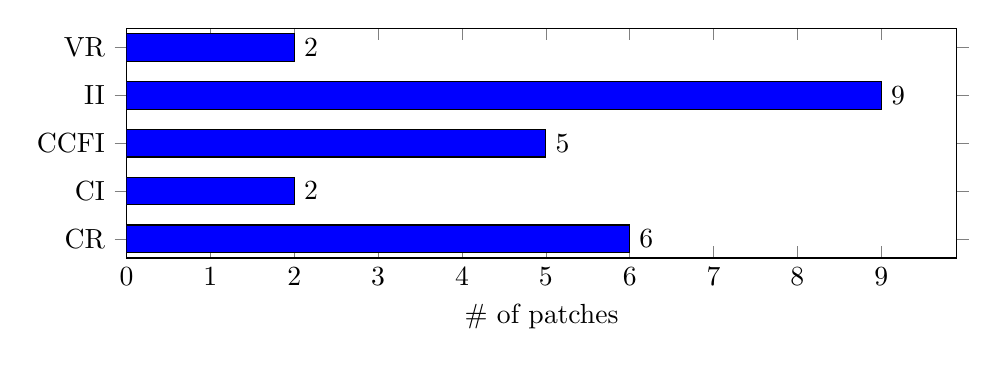
\begin{tikzpicture}
    \begin{axis}[
        xbar, xmin=0,
        xlabel={\# of patches},
        symbolic y coords={
            {CR},
            {CI},
            {CCFI},
            {II},
            VR
        },
        ytick=data,
        %y tick label style={rotate=30},
        nodes near coords,
        nodes near coords align={horizontal},
        height=4.5cm,
        width=\linewidth,
    ]
    \addplot[fill=blue] coordinates {
        (6,{CR})
        (2,{CI})
        (5,{CCFI})
        (9,{II})
        (2,VR)};
    \end{axis}
    \end{tikzpicture}
    \small \caption{Default SPR transformations}
    \label{figure:transforms-old}
\end{subfigure}
\hfill
\begin{subfigure}[b]{.48\linewidth}
    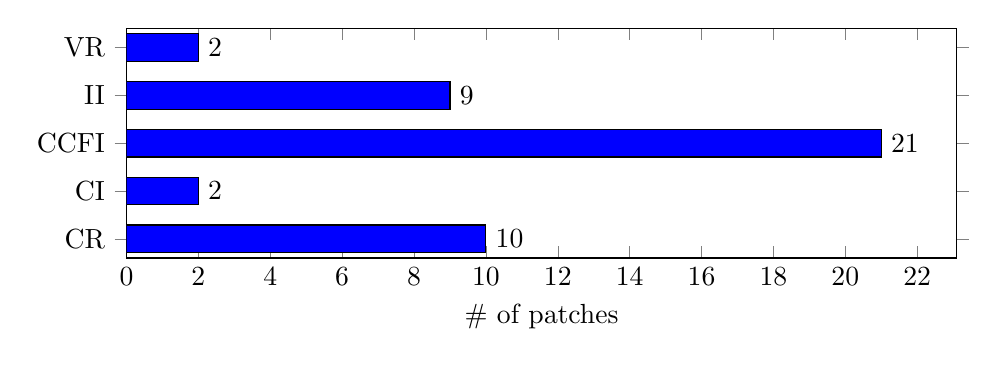
\begin{tikzpicture}
    \begin{axis}[
        xbar, xmin=0,
        xlabel={\# of patches},
        symbolic y coords={
            {CR},
            {CI},
            {CCFI},
            {II},
            VR
        },
        ytick=\empty,
        ytick=data,
        %y tick label style={rotate=30},
        nodes near coords,
        nodes near coords align={horizontal},
        height=4.5cm,
        width=\linewidth,
    ]
    \addplot[fill=blue] coordinates {
        (10,{CR})
        (2,{CI})
        (21,{CCFI})
        (9,{II})
        (2,VR)};
    \end{axis}
    \end{tikzpicture}
    \small \caption{Default + new SPR transformations}
    \label{figure:transforms-new}
\end{subfigure}

    \small \caption{Distribution of transformations employed in correct SPR patches. CR is Condition Refinement, CI is Condition Introduction, CCFI is Conditional Control Flow Introduction, II is Insert Initialization, VR is Value Replacement}
        \label{figure:transforms}
    \vspace{-0.2in}
\end{figure}

% Open access
In addition, we provide open access to the SQL database with the results of this empirical study\footnote{host: lt-pc1.uwaterloo.ca; DB name: cs858; user/pw: guest/guest}.
